\section{Introduction to radio interferometric imaging}\label{radio}
%This Section gives an introduction to radio interferometric imaging. We introduce how the interferometer measures visibilities, what problems arise and how reconstruction algorithms solve them. 

A radio interferometer consists of several antennas. Each antenna pair measures a visibility in Fourier space. Each measurement consists of an amplitude and phase at a location at a $u$ and $v$  location. The distance between the antennas, which we call the baseline, defines what point in the Fourier space gets sampled. The Figure \ref{radio:sampling:ants} shows the antenna layout of the MeerKAT radio interferometer, and the Figure \ref{radio:sampling:pattern} shows the measurement points in Fourier space. Short baselines sample points close to the origin, and contain the low-frequency Fourier components. They contain information about large areas of the images. Longer baselines measure points further away from the origin. They sample the high-frequency Fourier components. They contain information about edges, and other small structures in the image.


\begin{figure}[!h]
	\centering
	\begin{subfigure}[b]{0.49\linewidth}
		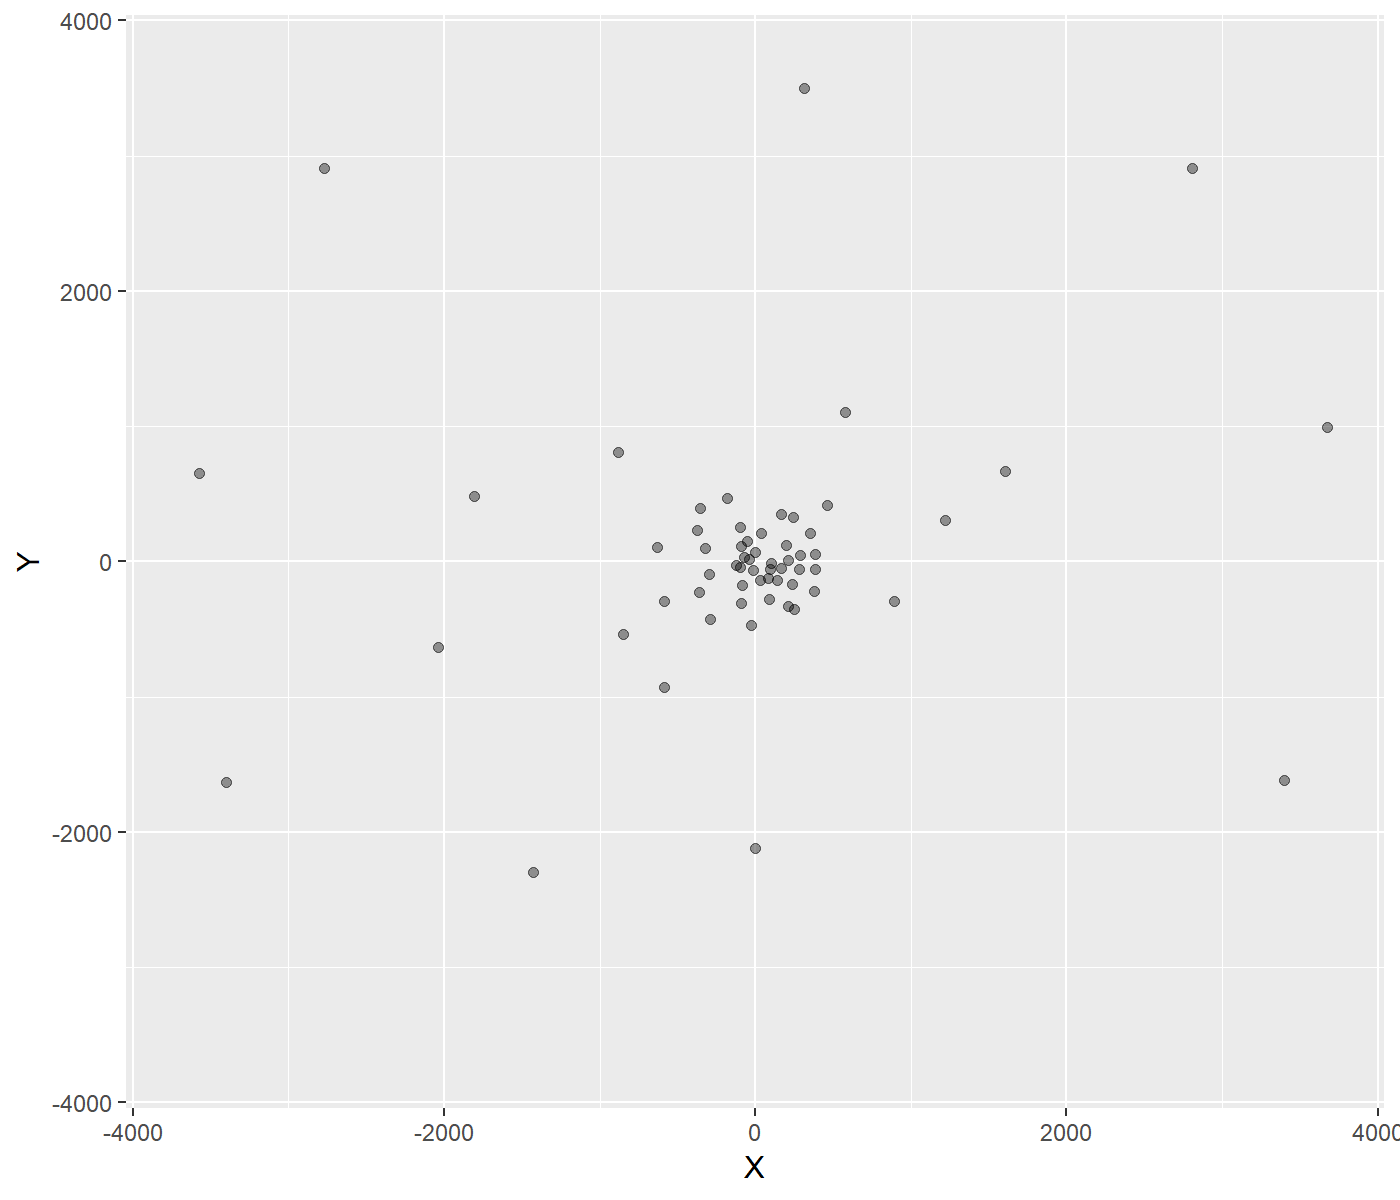
\includegraphics[width=\linewidth]{./chapters/01.intro/aperture/ants.png}
		\caption{Antenna layout.}
		\label{radio:sampling:ants}
	\end{subfigure}
	\begin{subfigure}[b]{0.49\linewidth}
		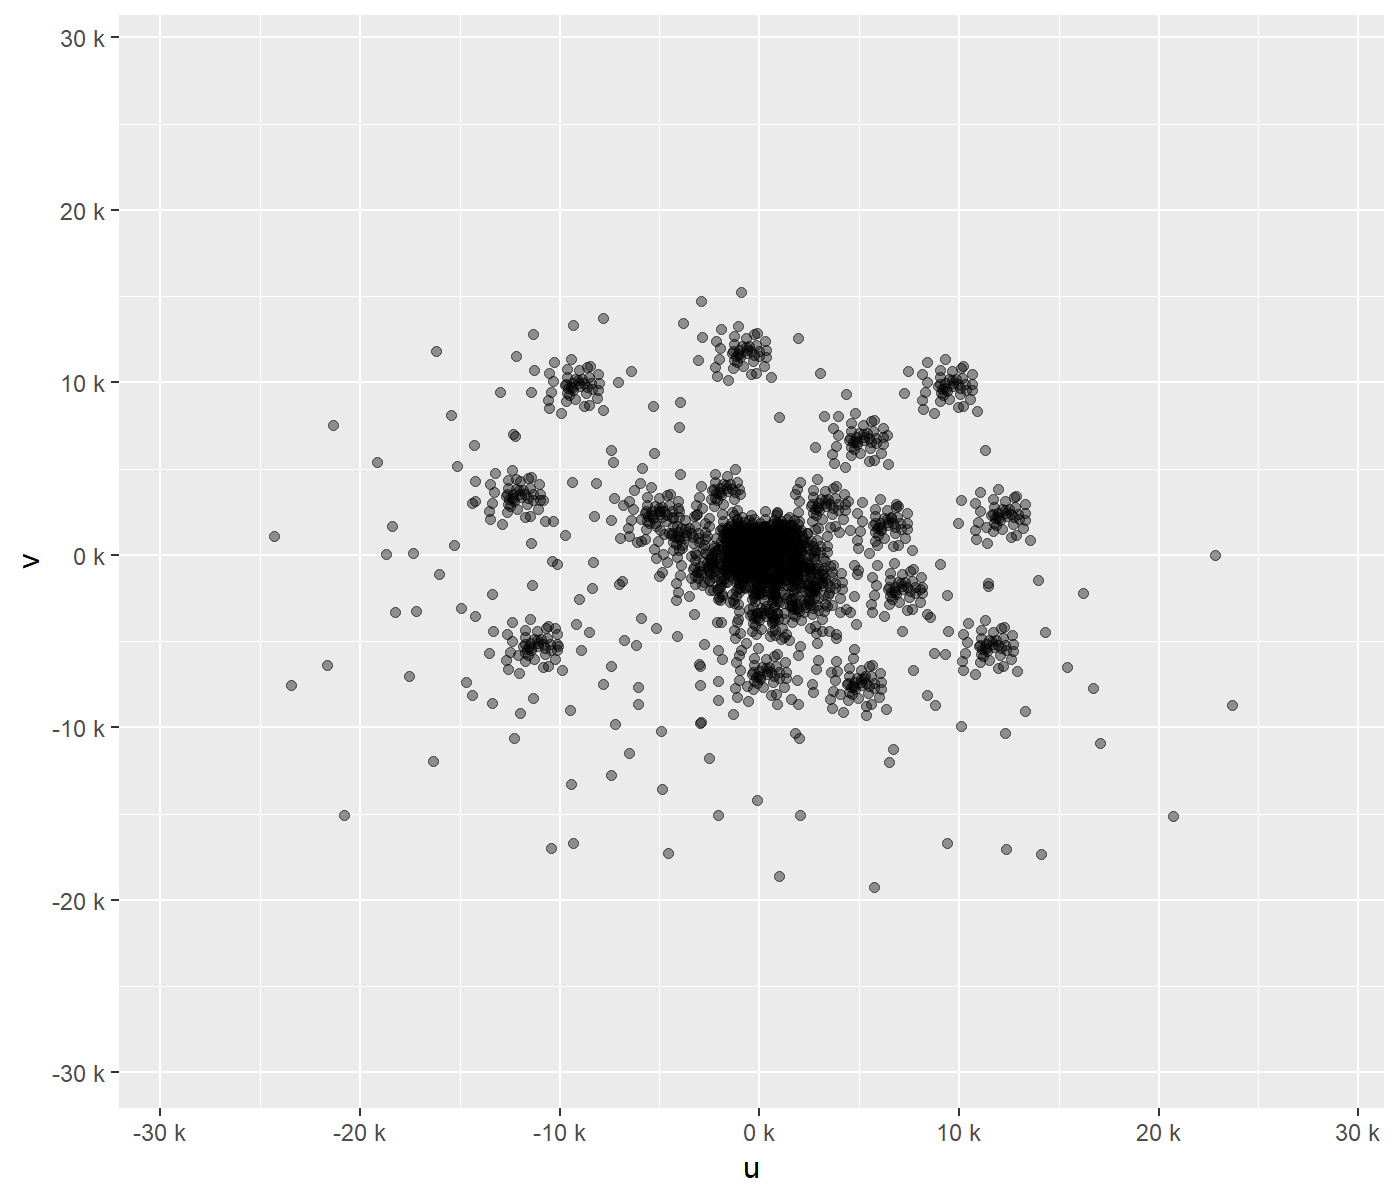
\includegraphics[width=\linewidth]{./chapters/01.intro/aperture/snapshot.png}
		\caption{Visibility sampling pattern.}
		\label{radio:sampling:pattern}
	\end{subfigure}
	\\
	\begin{subfigure}[b]{0.49\linewidth}
		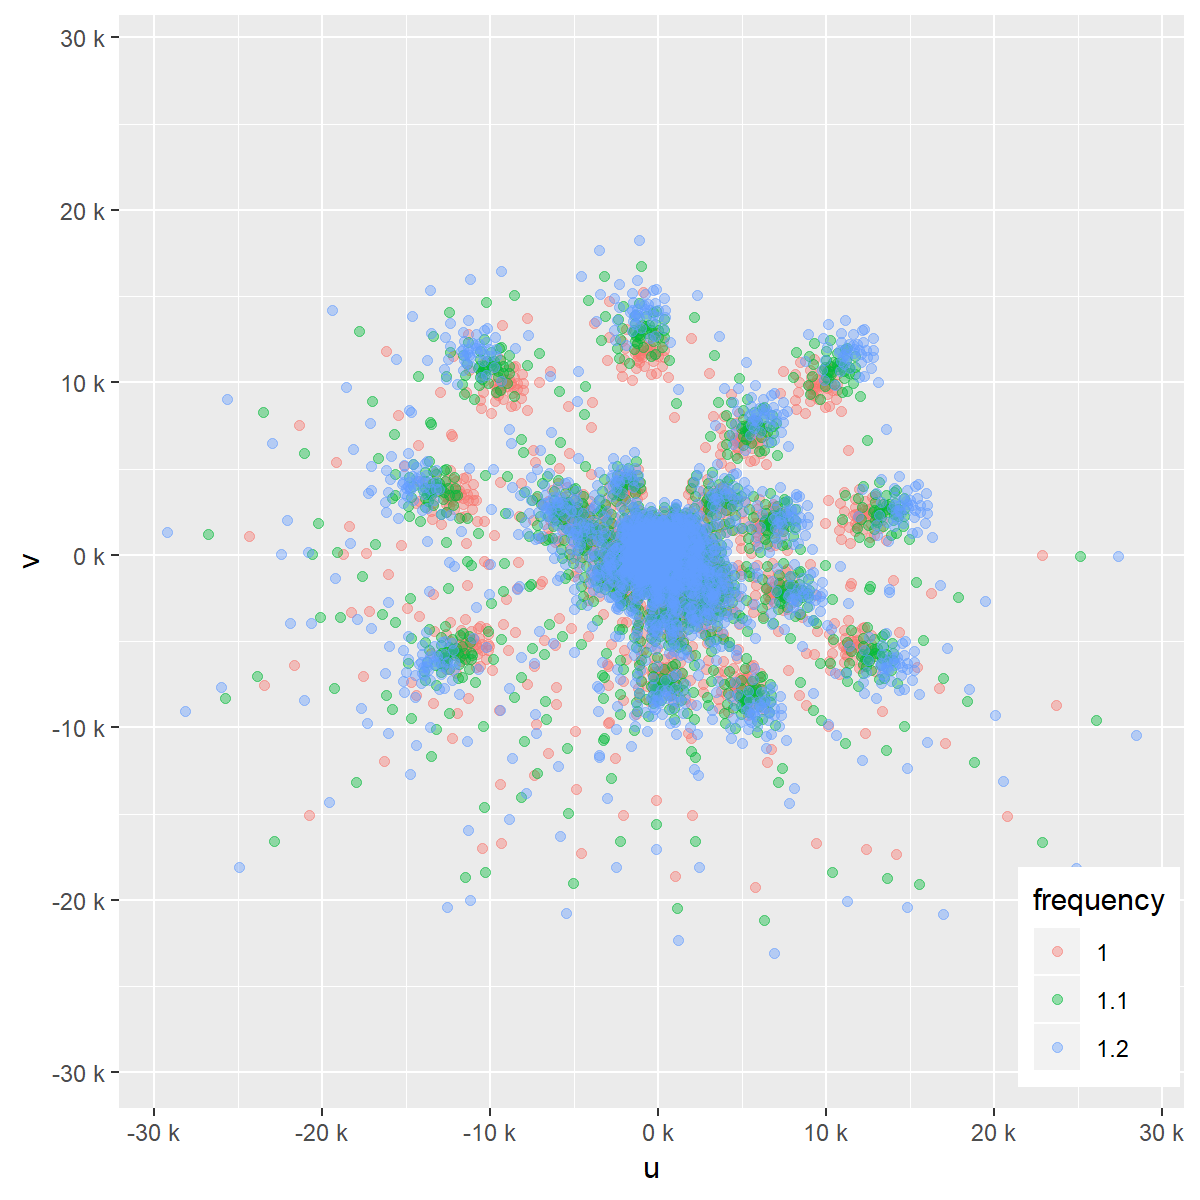
\includegraphics[width=\linewidth]{./chapters/01.intro/aperture/frequencies.png}
		\caption{Visibilities added from multiple channels.}
		\label{radio:sampling:freq}
	\end{subfigure}
	\begin{subfigure}[b]{0.49\linewidth}
		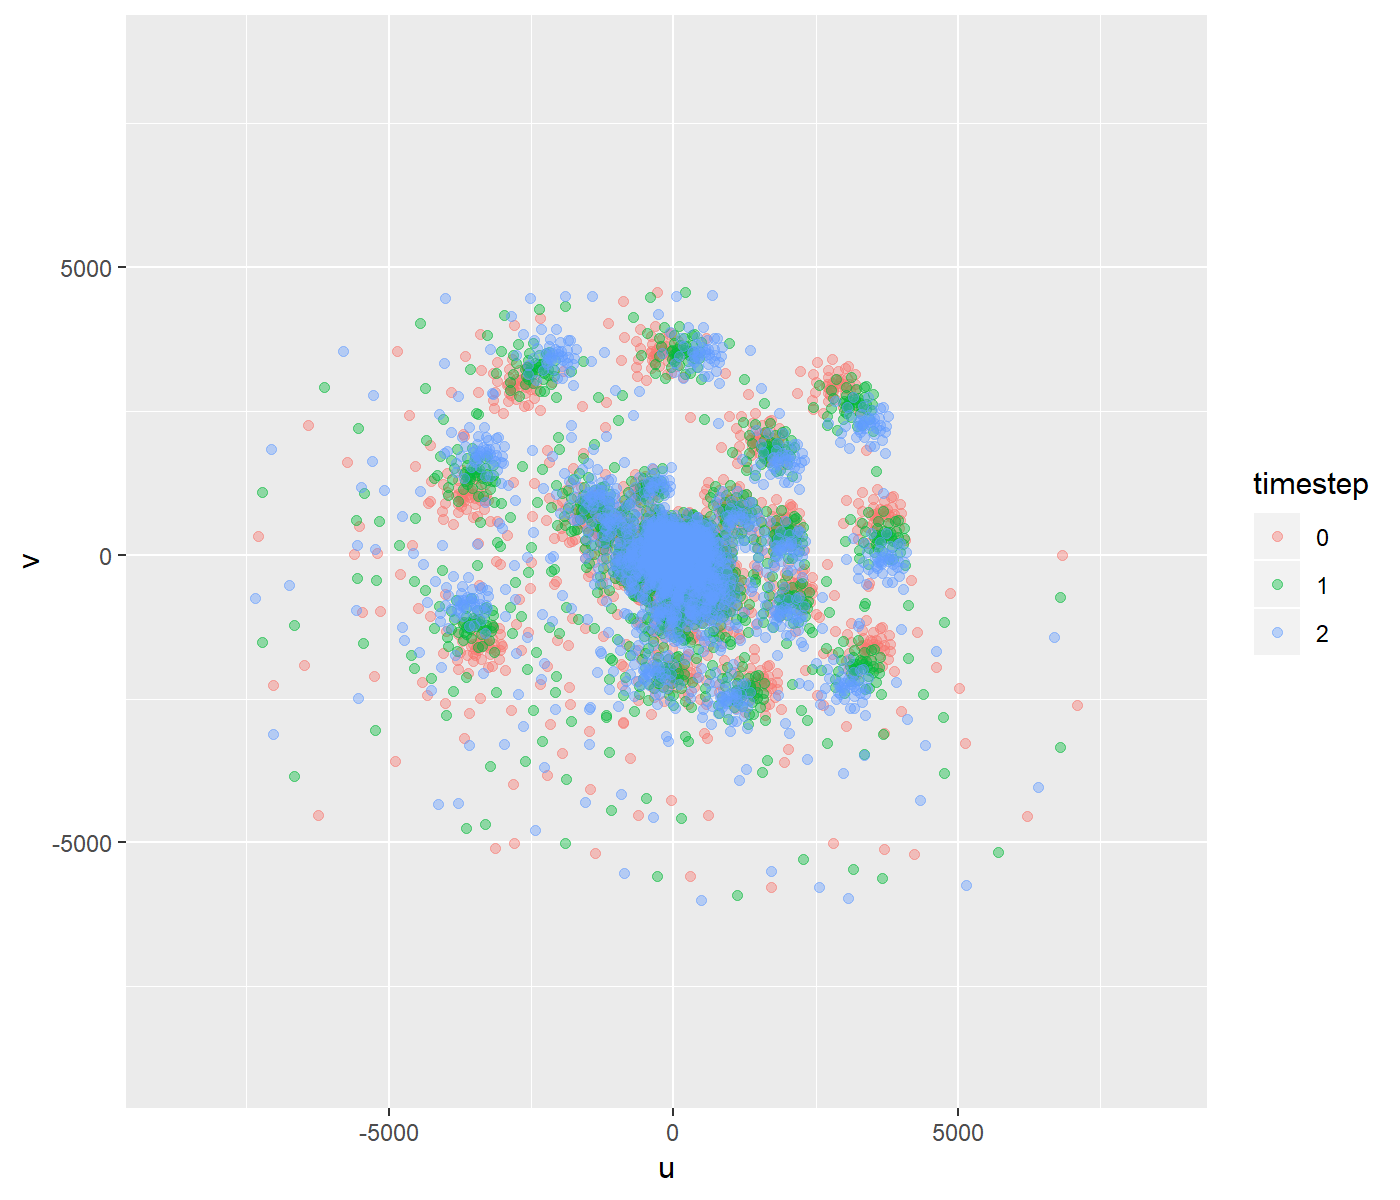
\includegraphics[width=\linewidth]{./chapters/01.intro/aperture/timesteps.png}
		\caption{Visibilities added from multiple timesteps.}
		\label{radio:sampling:time}
	\end{subfigure}
	
	\caption{Sampling regime of the MeerKAT radio interferometer.}
	\label{intro:sampling}
\end{figure}

The sampling pattern of the MeerKAT interferometer is not uniform in the Fourier space. We have areas which are densely sampled, and areas which are sparsely sampled. Note that we only have a few samples of the high-frequency Fourier components. We are missing measurements from a large portion of the Fourier space.

Radio interferometers use two "tricks" to measure more points in the Fourier space. Radio interferometers measure the sky in different radio channels simultaneously. We can add the visibility measurements from different channels together, shown in Figure \ref{radio:sampling:freq}. Each channel measures the Fourier space using the same pattern, but scaled by the radio frequency. 

The second trick is to use the earth's rotation to sample different points in the Fourier space. The earth's rotation also rotates the sampling pattern in Fourier space, shown in Figure \ref{radio:sampling:time}, and we can sample the Fourier space at new locations.

The MeerKAT radio interferometer measures 2016 visibilities, for each channel, at each timestep. It has 20 thousand radio channels. The time resolution can be as low as half a second. This results in roughly 80 million visibility measurements per second. In radio astronomy, we want to reconstruct several hours worth of visibility measurements. 
%GB and TB of data

\begin{figure}[htp]
	% preliminary
	\sbox\twosubbox{%
		\resizebox{\dimexpr.9\textwidth-1em}{!}{%
			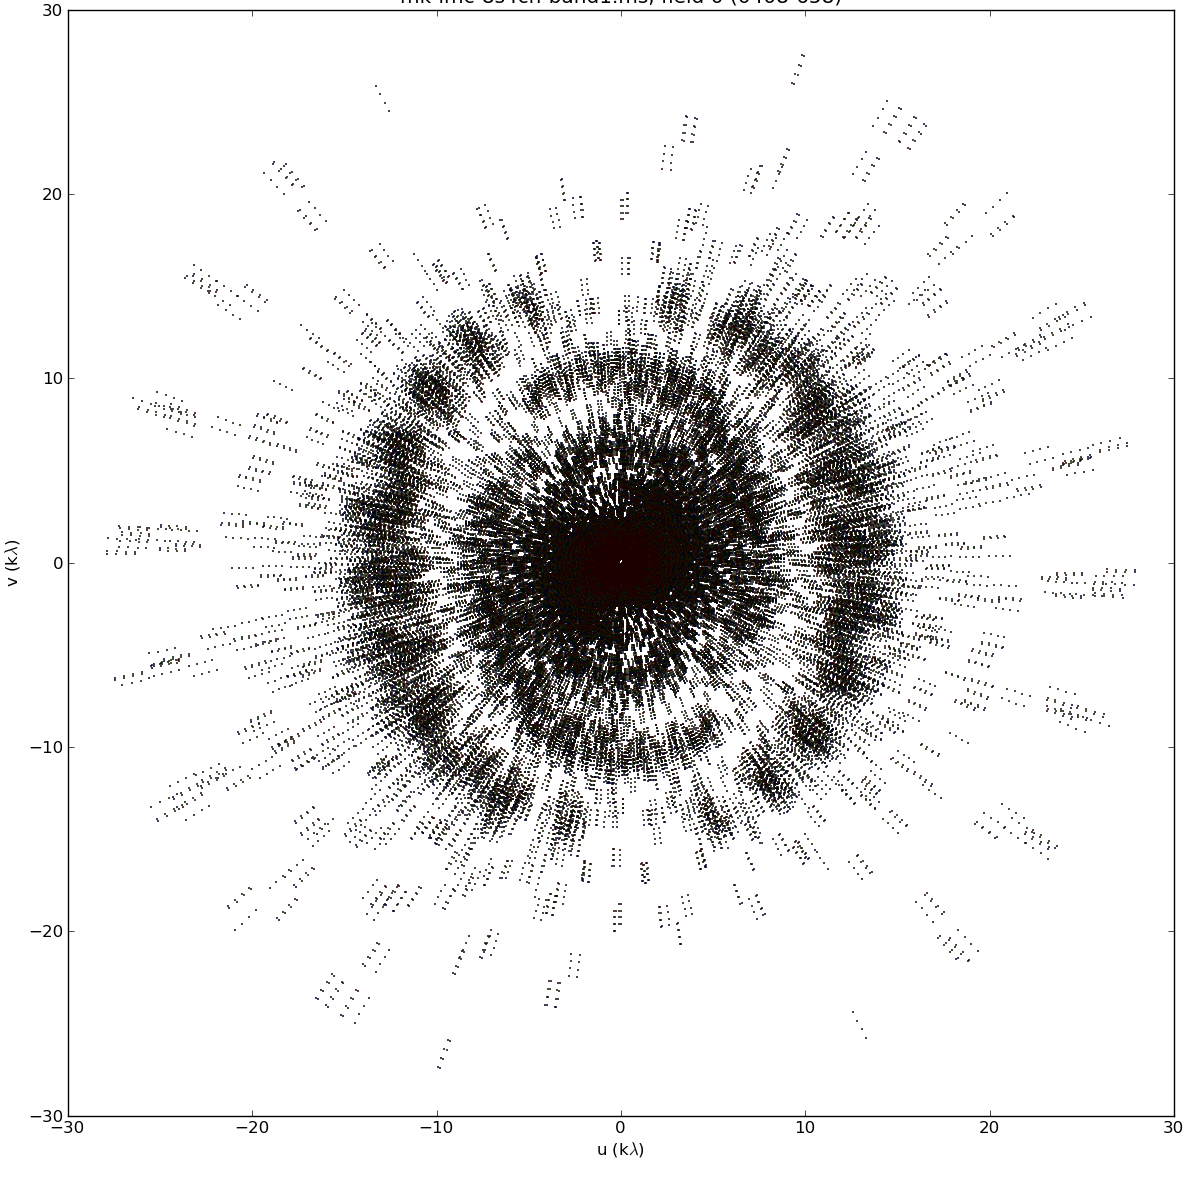
\includegraphics[height=3cm]{./chapters/01.intro/meerkat_uv2.png}%
			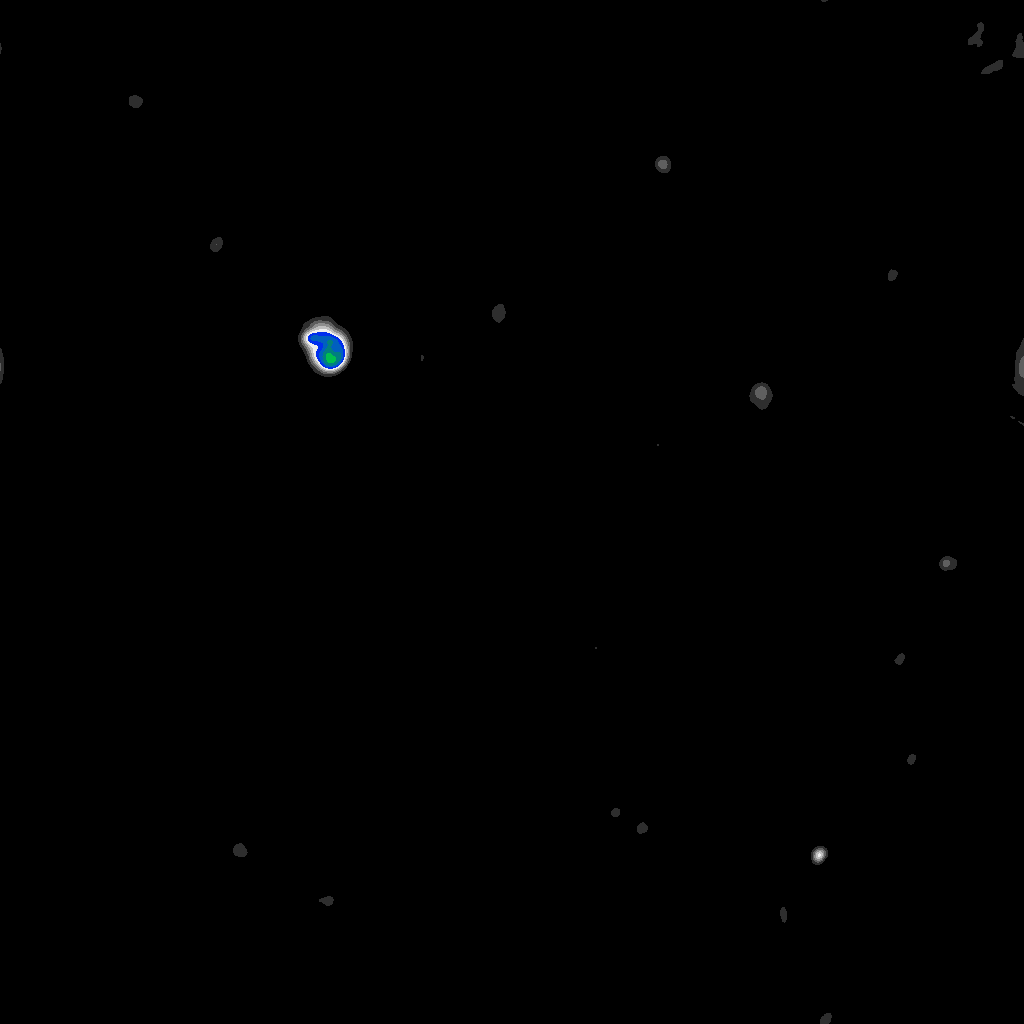
\includegraphics[height=3cm]{./chapters/01.intro/mk2/clean.png}%
		}%
	}
	\setlength{\twosubht}{\ht\twosubbox}
	
	% typeset
	\centering
	\subcaptionbox{Real-world visibilities combined from different channesl and timesteps.\label{intro:inversefig:uvspace}}{%
		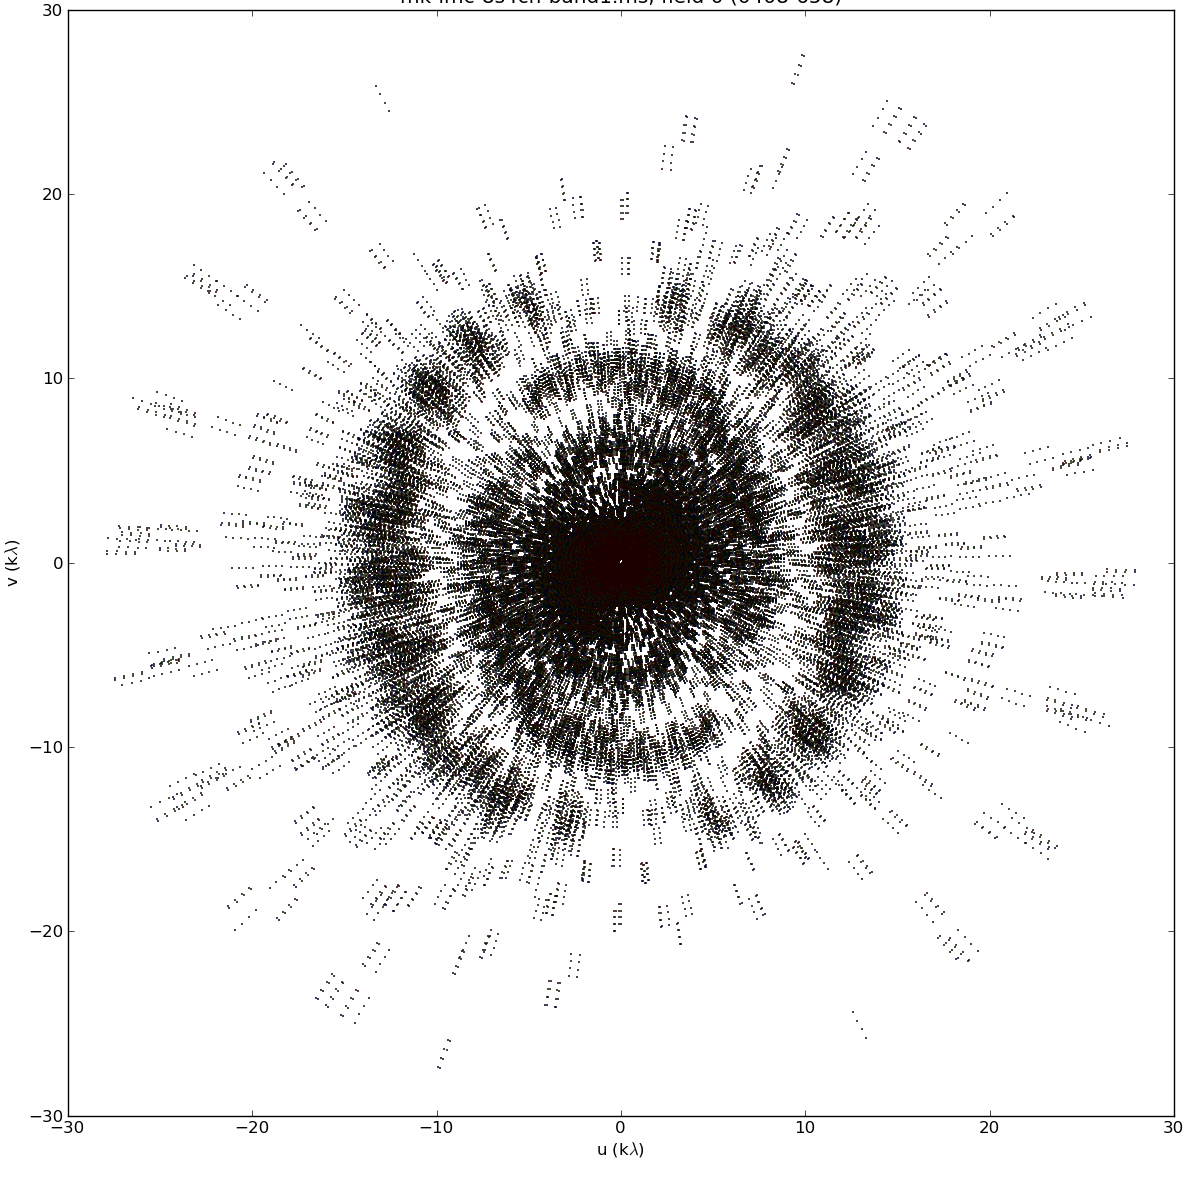
\includegraphics[height=\twosubht]{./chapters/01.intro/meerkat_uv2.png}%
	}\quad
	\subcaptionbox{Reconstruction of the visibility measurements.\label{intro:inversefig:reconstruction}}{%
		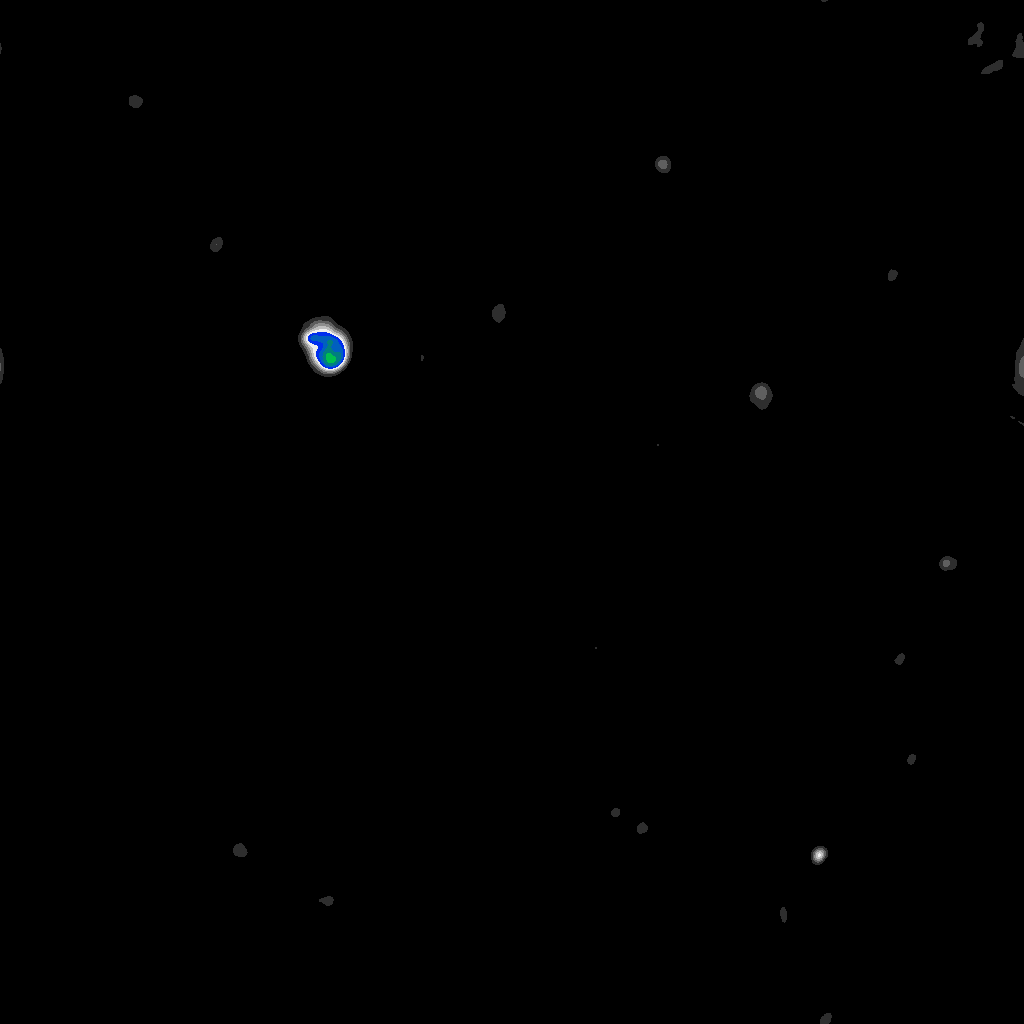
\includegraphics[height=\twosubht]{./chapters/01.intro/mk2/clean.png}%
	}
	\caption{Example of an image reconstruction for Fourier measurements of the MeerKAT radio interferometer}\label{intro:inversefig}
\end{figure}

It is easy to see that the visibility measurements from MeerKAT quickly fills up the hard disk and the Fourier space with samples. The Figure \ref{intro:inversefig:uvspace} shows a fraction of the visibility samples from a real-world observation. The visibilities are combined from multiple channels and multiple timesteps. Although we have a large number of visibilities, we still have areas of the Fourier space without a sample. Although we have a large number of samples, the visibilities are still an incomplete. From the measurements alone, we cannot reconstruct the image shown in Figure \ref{intro:inversefig:uvspace}.

This is known as an ill-posed inverse problem in the literature. A problem is considered ill-posed when:
\begin{enumerate}
	\item No solution exists.
	\item There are solutions, but no unique solution exists.
	\item The solution behavior does not change continuously with the initial condition (For example: a small change in the measurements lead to a very different reconstructed image).
\end{enumerate}
Image reconstruction for radio interferometer is an inverse problem, because we want to find the image which the interferometer observed in Fourier space. It is ill-posed in general, because there are many different images fitting the measurements.

Note that we can reduce the resolution of the reconstructed image until the problem becomes well-posed. The Nyquist-Shannon sampling theorem states the case of radio interferometers: The highest highest Fourier-frequency we measure should be more than twice the highest frequency in the image. The center of the Fourier space in Figure \ref{intro:inversefig:uvspace} is densely sampled. We can reconstruct a low-resolution image that only needs the information from the densely sampled center.

However, this would reduce the effective resolution of the reconstruction. If we can solve the ill-posed inverse problem, we would be able to retrieve the observed image at a higher resolution than possible with the Nyquist-Shannon sampling theorem. As it turns out, this is possible to solve the ill-posed inverse problem by including prior information. We use a numerical optimization algorithm and find the optimal image, which is both consistent with the measurements and consistent with our prior knowledge. This is known in signal processing as compressed sensing \cite{candes2006robust,donoho2006compressed} in the literature. The theory of Compressed Sensing shows that, under the right prior information, we are guaranteed to reconstruct the observed image at a higher resolution than under the Nyquist-Shannon sampling theorem.

%In Section \ref{intro2:ill-posed}, we introduce the Compressed Sensing sampling theorem and show how it works in the case of radio interferometric image reconstruction. The Section \ref{intro2:rec} shows how we can use the theory to create a reconstruction algorithm in practice. But first, we dive deeper into the odds and ends of radio interferometry. 

\subsection{The theory of Compressed Sensing}\label{radio:cs}
We introduce the theory of Compressed Sensing for the problem of radio interferometric image reconstruction. As we have mentioned compressed sensing image reconstruction involves a numerical optimization algorithm to find the optimal solution which is consistent with our measurements and consistent with our prior knowledge. As we will see later, the theory of compressed sensing guarantees us exact reconstruction under certain assumptions. 

Let us formulate the image reconstruction as an optimization problem.The image reconstruction wants to to find the image which is as close to the measurements as possible. Or more formally, we want to minimize the euclidean distance between the visibility measurements $V$ and the reconstructed image $x$. We write it as an objective function:

\begin{equation}\label{radio:cs:l2}
\underset{x}{minimize} \: \left \| V - Fx \right \|_2^2
\end{equation}

We can reconstruct the image by finding the optimum of the objective function \eqref{radio:cs:l2}. The objective function is convex, meaning it has only one global minimum, and we can use the class of convex optimization algorithms to search the minimum. However, our measurements $V$ are incomplete, meaning we do not have all the data we need for reconstruction. This means our objective function \eqref{radio:cs:l2} does not "point" to the observed image. It still has a global minimum, but observed image is not guaranteed to be near the global minimum.

A side note: We are guaranteed to find the observed image at the minimum of \eqref{radio:cs:l2} is when the measurements fulfill the Nyquist-Shannon sampling theorem. In that case, we can find the minimum by calculating the inverse Fourier transform: $x = F^{-1}V$. We can still calculate the inverse Fourier transform when we are dealing with incomplete measurements, but it does not result in the observed image.

However, the objective \eqref{radio:cs:l2} only includes information about the measurements. As we have mentioned before, we have prior knowledge about the image. We know it is likely to contain stars. Stars are radio-emissions which are concentrated around a single pixel. In that case, most pixels of the image will be zero, except for the locations where the interferometer has located stars. In other words, we know that the image is sparse. We can add a regularization to the objective function \eqref{radio:cs:l2} and force the reconstructed image to be sparse. This results in the modified objective function:

\begin{equation}\label{radio:cs:lasso}
\underset{x}{minimize} \: \left \| V - Fx \right \|_2^2 + \lambda \left \| x \right \|_1
\end{equation}

Note the two terms in the objective \eqref{radio:cs:lasso}: We have the same term from our measurements, which we call the "data term". But we also have an additional "regularization term", which is the L1 norm\footnote{Sum of absolute values of the pixels} and forces our reconstruction to be sparse. The parameter $\lambda$ represents how much emphasis we put on the regularization. The new objective function is still convex, it still has a global minimum. The regularization term simply shifted the global minimum to a different location when compared to the first objective \eqref{radio:cs:l2}. Now the question is: How likely is our modified objective \eqref{radio:cs:lasso} to point at the observed image? The theory of Compressed Sensing tells us that it depends on the image content of the observed image. If it only consists of stars, we are practically guaranteed to find the observed image at the minimum of \eqref{radio:cs:lasso}, even though we are dealing with incomplete measurements.

We use the words 'practically guaranteed' because the theory of Compressed Sensing does give us guarantees to find the observed image at the minimum of \eqref{radio:cs:lasso} under certain assumptions. The issue is these assumptions are hard to verify for any given reconstruction problem. In reality, it is often easier to empirically show that the regularization works. For example, by creating a super-resolved\footnote{The radio interferometer also has a resolution limit. Super-resolved reconstructions were able to find structures which are smaller than the limit of the instrument.} reconstruction from visibility measurements \cite{dabbech2018cygnus}. The assumptions do have important implications for instrument design. This project however is focused on the numerical optimization algorithm. We do not have an influence on the visibility measurements, for our intends and purposes, the measurements are fixed. That is why we first give an intuitive explanation to when the observed image is at the minimum of the objective \eqref{radio:cs:lasso}, and what this means for the ill-posed image reconstruction in Section \ref{radio:cd:intuitive}. Then we give an overview of the formal guarantees in Section \ref{radio:cd:formal} and the implications for the visibility measurements.


\subsubsection{Intuitive explanation of Compressed Sensing}\label{radio:cd:intuitive}
We go back to 

Intuitive

Why it works

Here we see the core assumption for the theory of Compressed Sensing to apply: We know what the observed image looks like, and can model it adequately as a regularization term. This is not always true. We do only know what the observed image looks like to a certain degree, and the regularization term does not model the observed image perfectly. In our example, we assume the image is sparse, because it only contains point sources. This is not always true in reality, as radio interferometers also measure extended emission like hydrogen clouds, which span over several pixels. The observed image will not be as sparse as before. In that case we can still try to find the observed image with an L1 regularization, but we may need more visibility measurements for the reconstruction.

To guarantee the observed image is at the There are more assumptions involved about the properties of the visibility measurements. 

There are other regularization methods that model both point sources and extended emissions \cite{starck2003astronomical, starck2015starlet}. With these regularizations, we can reconstruct the observed image from fewer measurements, or find a super-resolved image from the same measurements. This means that the number of samples which are necessary for reconstruction depend on the regularization we use.

The theory of Compressed Sensing can a
To solve the ill-posed inverse problem, we have an implicit data modeling task involved. We need less visibility measurements the better we can model the observed image.

The theory of Compressed Sensing gives us a formula to how many samples we need for the reconstruction. Sadly, these are based on hard-to-verify assumptions. 

Where is the limit
Ther is one, but we cannot calculate the limit in practice. It is based on assumptions hard-to-verify assumptions. In reality, it is often easier just to find the reconstruction and do an empirical proof. Our regularization works, because it produces good results.



First assumption: we know what the observed image looks like. Not always true, radio interferometers also measure hydrogen clouds, which span an area over several pixels.
We can retrieve an image below the Nyquist-Shannon sampling rate. Where is the limit? how many samples do we need to retrieve the image? In short: There is a limit, but it is based on even harder to prove assumptions. We quickly introduce them for completion's sake.

In practice, we know this works, because it was shown to work.

This project does not dive deeper into the prior, and how good it models the observed image. We are diving into numerical optimization algorithms and how we can retrieve the observed image with a given regularization.




So when we have a good prior, the objective points to the observed image even though we do not have enough samples according to the Nyquist-Shannon theorem. What the theory of Compressed Sensing can tell us is how many samples we need until the objective points to the observed image.

Sadly, we cannot verify that the assumptions hold in practice. is that we cannot verify these assumptions in practice.


Depends on the image content and the prior we use. Also, the theory of Compressed Sensing difficult bounds in practice.




Theory of Compressed Sensing
Pretty well, if the image only contains stars. Theory of compressed sensing 
Incoherence. We gain maximum information about the non-zero locations with each visibility measurement.

All we need for Compressive Sensing: A reconstruction space which our image is sparse.
A measurement space which is incoherent to our reconstruction space.

Then the number of samples we need does not depend on the resolution of the image, but on the number of non-zero components in our reconstruction space.





\subsubsection{Formal Guarantees}\label{radio:cd:formal}
RIP
What is the RIP
Meaning of $F$. How many random columns of F are uncorrelated? Remember that we have redundant information, the whole matrix $F$ does have columns which are correlated.

At what point are we guaranteed? The matrix $A$ needs to fullfil the Restricted Isometry Porperty (RIP) \cite{candes2006robust,donoho2006compressed}.
Approximately orthonormal on sparse signals. (If we randomly choose ten columns of $F$, how much do they correlate. We want as little correlation as possible.)
Calculate the RIP is NP-hard\cite{tillmann2013computational}. Approximations are also difficult to compute\cite{natarajan2014computational}.
So we can only talk about how likely a given matrix fullfils the RIP. Matrix where each element is sampled from a random Gaussian distributîon has the highest change.

Random samples in the Fourier space also have a high chance to fulfill the RIP \cite{haviv2017restricted}.

Not possible for Radio interferometers, because they sample in the Fourier space. Not random.

There are also extended emissions, clouds etc. Resulting in a lot of non-zero pixels. There may be better sparse spaces for radio astronomy.

But also RIP may be too strict. Exact reconstruction can also work under less strict conditions\cite{candes2011probabilistic} active field of research.

We do not know if the image we reconstruct is the observed one. Calculating good bounds are hard. 
Demonstrated super-resolution performance.


\subsubsection{General Compressed Sensing reconstruction formulation}
Use everything with the L1 norm. More general formulation

$F$ is fixed, because we cannot change the interferometer.

We do just need a sparse space.





T 

So far, we discussed how the interferometer measures in Fourier space, and we wish to find the observed image that matches the measurements. In other words, we wish to find a solution to a system of linear equation \eqref{intro2:ill-posed:linear}, where $V$ are the measurements, $x$ is the observed image and $F$ is the Fourier transform matrix. We also discussed that $F$ can be complicated in practice, but is still essentially a linear operator. Meaning we know how the inverse Fourier transform matrix $F^{-1}$, and the question arises: Why can't we solve the equations \eqref{intro2:ill-posed:linear} by calculating the inverse Fourier transform? Or, why does $x = F^{-1} V$ not lead to the observed image?



The answer is, the equations \eqref{intro2:ill-posed:linear} do not have a unique solution, which makes the problem ill-posed. The problem is considered ill-posed when it has one of the following properties:
\begin{enumerate}
	\item No solution exists.
	\item There are solutions, but no unique solution exists.
	\item The solution behaviour does not change continuously with the initial condition (For example: a small change in the measurements lead to a very different reconstructed image).
\end{enumerate}
From linear algebra, we know that an under-determined system of linear equations, i.e. when \eqref{intro2:ill-posed:linear} has more pixels than visibility measurements, then the problem is under-determined and there may be a potentially infinite number of solutions to the system. Under-determined systems arise in many similar fields, as for example in X-Ray imaging of the sun\cite{felix2017compressed}. However, radio interferometers measure a large number of visibilities. We generally have more visibilities than pixels. This means the image reconstruction problem \eqref{intro2:ill-posed:linear} for radio interferometers is actually over-determined.

From linear algebra, we know that an over-determined system either has one or zero solutions. At first glance it may be counter-intuitive why there are many possible solutions to \eqref{intro2:ill-posed:linear} for radio interferometers. The reason why lies in two properties of the measurements: They are noisy and incomplete.

The radio interferometer measures noisy visibilities, meaning each amplitude and phase of a measurement is influenced by an unknown noise factor. Finding a reconstructed image is the same as finding the de-noised versions of the visibility measurements. This alone would make the problem ill-posed, but the visibilities actually have a second property that makes them ill-posed: incompleteness.

When we look back at figure \ref{intro:inversefig:uvspace}, it is clear to see that the interferometer does not sample the visibilities in a uniform way. There are regions with a high sample density. The density decreases when we move further away from the center. The higher frequency visibilities get fewer and fewer samples. This means we are missing data for crucial measurements for the reconstruction.

Also note that the question whether the measurements are incomplete essentially comes down to the image resolution of the reconstruction: Since we are missing high-frequency measurements and we can choose the resolution of the image, we can also reduce the resolution of the reconstructed image until the missing frequencies become negligible. However, if we can solve the ill-posed inverse problem, we can reconstruct an image at a higher resolution from the same measurements. The question is how do we solve the ill-posed inverse problem?

\subsubsection{Adding a regularization} \label{intro:linear:regularization}
For ill-posed inverse problems, there are two viewpoints for the same idea. From the viewpoint of optimization, we can solve the ill-posed image reconstruction problem \eqref{intro:linear:linear} by adding a regularization. The regularization creates a system of linear equations with a unique solution. From the viewpoint of Bayesian Statistics, we include prior knowledge about the image, and therefore search the most likely image given the measurements. For this project, both terms describe the same idea and we use regularization and prior interchangeably. We know that the reconstructed image from radio interferometers contain a mixture of stars (point sources located in a single pixel) and extended emissions like hydrogen clouds. By adding this prior knowledge to the reconstruction problem, we can find the most likely image given the measurements. As we will see, under the right prior, we can create a reconstruction algorithm that is almost guaranteed to find the truly observed image in theory.

There are different ways to include regularization in the reconstruction problem. In this project, we use the following method: We cast the image reconstruction problem into an optimization objective consisting of a data fidelity term and a regularization term. A reconstruction algorithm therefore consists of an optimization objective, a prior function and an optimization algorithm.

\begin{equation}\label{intro:linear:compressed}
\underset{x}{minimize} \: \left \| V - Fx \right \|_2^2 + \lambda P(x)
\end{equation}

The objective \eqref{intro:linear:compressed} has a data term $\left \| V - Fx \right \|_2^2$, which forces the most likely image to be as close to the measurements as possible, and the regularization term $P(x)$, which penalizes unlikely images according to our prior function. The parameter $\lambda$ represents how much we penalize unlikely images and by extend, much noise we expect in the reconstruction. The parameter $\lambda$ is either left to the user to define, can be estimated from the data \cite{miller1970least}. 

The prior function $P()$ represents our prior knowledge about the image. It assigns a high penalty for unlikely images. In in radio interferometric image reconstructions tend to use similar prior functions as for image de-noising applications. Such as: Total Variation ($\left \| \triangledown x \right \|_1$) \cite{wiaux2009compressed}, L2 ($\left \|x \right \|_2$) \cite{ferrari2014distributed} or the L1 norm in a wavelet space ($\left \|\Psi x \right \|_1$) \cite{girard2015sparse}.

Finally, an optimization algorithm is necessary which can optimize the objective function \eqref{intro:linear:compressed} with the chosen prior function $P()$. Typical choices for optimization algorithms in image reconstructions are Interior Point Methods like Simplex, Matching Pursuit \cite{hogbom1974aperture} and ADMM\cite{carrillo2014purify}. 

A reconstruction algorithm for radio astronomy consists of an optimization objective, a prior function and an optimization algorithm. It is a three dimensional design space. Not every prior is suitable for every optimization algorithm. The choice of optimization objective influences both what prior and what optimization algorithm we can use. Although there are a different choices for the optimization objective, we limit ourselves to the objective \eqref{intro:linear:compressed} and explore how we can distribute the reconstruction problem.

The last question that remains is, how close are the most likely image, under a given prior, to the truly observed one? Remember that the Nyquist-Shannon sampling theorem states that our uniform sampling frequency needs to be larger than twice the highest frequency in a band-limited signal\footnote{For example: if we want to record human voices with the highest frequency of 20 kHz, Nyquist-Shannon states our uniform sampling frequency has to be larger than 40 kHz to guarantee exact reconstruction}, and then the theorem guarantees exact reconstruction. For radio astronomy, we do not have uniformly sampled visibilities, and although we have a large number of samples, we are missing crucial parts of the Fourier space. Luckily, there is another sampling theorem that, under certain assumptions, guarantees exact reconstruction for the case of radio interferometers: The theory of compressed sensing.

\subsubsection{Compressive sampling of the sky}
For the sake of demonstration, let us assume the radio interferometer observes a patch of sky containing ten stars. It measures an incomplete set of random Fourier components of the ten stars, and we would like to reconstruct an image of size $256^2$ pixels. The emissions from stars are concentrated into a single pixel. For compressive sampling, we need to know an space in which our reconstructed image is sparse, and we need to take measurements in a different, incoherent space.

Our reconstructed image contains only zero pixels except at the ten locations of the stars, meaning the image space for this patch of the sky is already sparse. In this case, we do not need any additional sparse space like wavelets. We can reconstruct directly in the sparse image space, and we have the first requirement met for compressive sampling. 

The next requirement is that the measurement and reconstruction space (which is the image in this example), are as incoherent as possible. 

Yes, incoherence.
\begin{equation}\label{intro:linear:compressed2}
\underset{x}{minimize} \: \left \| V - Fx \right \|_2^2 + \lambda \left \| x \right \|_1
\end{equation}


Intuitively, the number of samples depend on the information content, not on the bandwidth. thi


At what point are we guaranteed? The matrix $A$ needs to fullfil the Restricted Isometry Porperty (RIP) \cite{candes2006robust,donoho2006compressed}.
Approximately orthonormal on sparse signals. (If we randomly choose ten columns of $F$, how much do they correlate. We want as little correlation as possible.)
Calculate the RIP is NP-hard\cite{tillmann2013computational}. Approximations are also difficult to compute\cite{natarajan2014computational}.
So we can only talk about how likely a given matrix fullfils the RIP. Matrix where each element is sampled from a random Gaussian distributîon has the highest change.

Random samples in the Fourier space also have a high chance to fulfill the RIP \cite{haviv2017restricted}.

Not possible for Radio interferometers, because they sample in the Fourier space. Not random.

There are also extended emissions, clouds etc. Resulting in a lot of non-zero pixels. There may be better sparse spaces for radio astronomy.

But also RIP may be too strict. Exact reconstruction can also work under less strict conditions\cite{candes2011probabilistic} active field of research.

\subsubsection{Reconstruction guarantees in the real world}

What does this all mean for image reconstruction?
For us, we design reconstruction algorithms and cannot influence the matrix $F$. We do not know if it actually 

The theory of compressed sensing gives us a framework. There is a data modelling task, and a task for finding efficient algorithms.

So there is a data modelling task in finding a good sparse prior.
We also do not know the proper sparse space in which radio interferometric images. We know several spaces, Curvelets \cite{starck2003astronomical} Starlets \cite{starck2015starlet}, Daubechies wavelets \cite{carrillo2012sparsity}. As of the time of writing, it is currently unknown which leads to the best reconstruction.
We can also learn dictionaries.

The task for efficient algorithms is finding the best way to optimize the objective with a given prior on real hardware. Fast convergence. Also difficult, because in practice the choice of prior can also influence convergence.


Compressed sensing based reconstruction algorithm. In radio astronomy.



\subsection{Noise, approximations and other difficulties in radio interferometry}
We give a short introduction into how the electromagnetic wave gets measured by the interferometer, turned into visibilities and finally processed into an image. Figure \ref{intro:system} shows a radio source and its electro-magnetic (em) wave arriving at the antennas of the interferometer. It then shows the three processes involved to arrive at an image: Correlation, calibration and image reconstruction.
	
\begin{figure}[h]
	\centering
	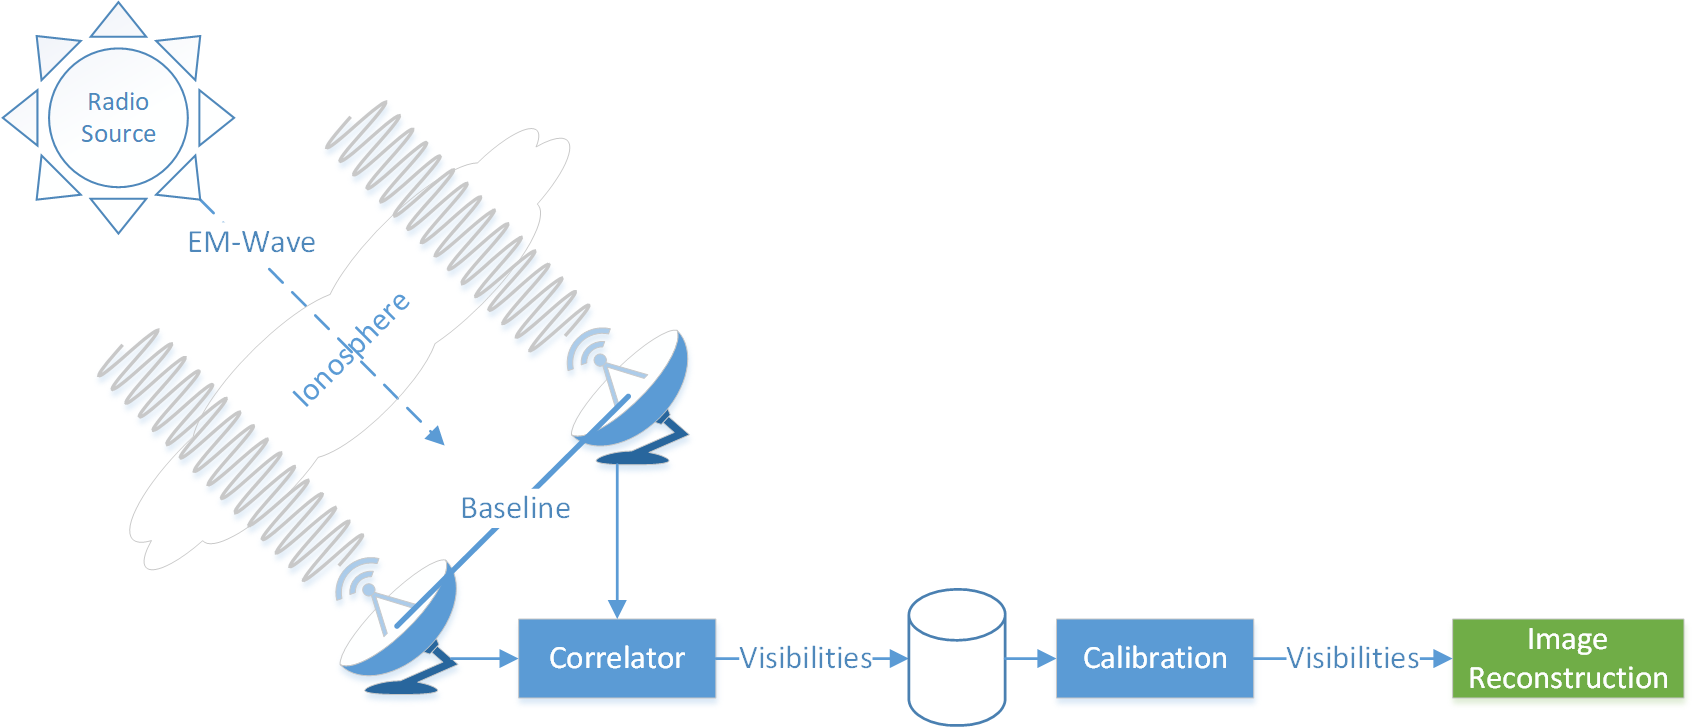
\includegraphics[width=0.80\linewidth]{./chapters/01.intro/system.png}
	\caption{Radio interferometer system}
	\label{intro:system}
\end{figure}

First, we have a source in the sky that is emitting em-waves in the radio frequency. The waves travel to earth, through the earth's ionosphere and finally to our interferometer. Along its path, the e-m waves may get distorted from various sources. For example, it may receive a phase shift by the ionosphere.

Then, the em-wave arrives at our interferometer. We call each antenna pair a baseline. Each baseline will end up measuring a single visibility. The distance between the antennas and their orientation to the em-wave will determine where we sample the $uv$-plane. Short baselines measure the $uv$-plane close at the origin, while long baselines sample the $uv$-space further away from the origin. Remember that the samples away from the $uv$-origin contain the information about edges and other details of our image. With a longer baseline the interferometer measures more highly resolved details, regardless of the antenna dish-diameter\footnote{Remember that this is the reason why we build radio interferometers. We do not need impossibly large dish diameters for a high angular resolution. We just need large distances between smaller antennas.}. The figure \ref{intro:system} shows the em-wave arriving at a single baseline of the interferometer. Each antenna picks up its version of the em-wave and transfers it to the correlator.

The correlator then takes the feed of each antenna and correlates the signals, which results in the amplitude and phase of the visibility component. Amplitude and phase for each visibility are measured for a short time range (i.e. fractions of a second up to several seconds). At this point, the visibilities are saved to disk for further processing. The radio interferometer produces a visibility measurement for each baseline, for each time range, for each frequency channel of the instrument. Because a single observation can take up to several hours, measured with several thousand frequency channels, radio interferometers produce an almost arbitrary large number of visibilities.

Calibration

Image Reconstruction

%Calibration. Effects from the ionosphere. Imperfections of the instrument, like varying antenna sensitivity.
%Calibration is complex, and not part of the project

%Image reconstruction generally happens after calibration. The focus of this project.
%self-calibration

\subsubsection{The measurement equation}
As we discussed so far, the radio interferometer measures visibilities of the sky image, and we wish to find the observed image from the measurements. Put formally, we wish to invert the following system of linear equations \eqref{intro2:model:linear}, where $V$ is the visibility vector\footnote{We use the lower-case $v$ to denote the axis in the Fourier space $uvw$, and the upper-case letter to denote the visibility vector.}, $F$ is the Fourier transform matrix and $I$ is the pixel vector of the observed image.

\begin{equation}\label{intro2:model:linear}
V = F I
\end{equation}

We wish to find the observed image $I$, while we only know the visibility vector $V$ and the Fourier transform matrix $F$. This is what we call the measurement equation. In most context for this project, looking is an adequate view of the image reconstruction problem. We will show why we cannot find the observed image $I$ by simply calculating the inverse Fourier transform. However, when we need to efficiently apply the Fourier transform, we need to know $F$ in more detail. As we will see, radio interferometers have some difficulties hidden in the Fourier transform matrix, which are difficult to handle efficiently. First, let us abandon the vector notation of \eqref{intro2:model:linear}, and represent the measurement equation with integrals \eqref{intro2:model:smallfov}.

\begin{equation}\label{intro2:model:smallfov}
V(u, v) = \int\int I(l, m)  e^{2 \pi i [ul+vm]} \: dl \: dm
\end{equation}

This is essentially the same problem. The main difference is that we do not represent the Fourier transform as a matrix $F$, but as integrals $\int\int e^{2 \pi i [ul+vm]}$, where $u$, $v$ are the coordinates in Fourier space and $l$, $m$ are the angles away from the image center. A single pixel represents the intensity of the radio emission from the direction $l$, $m$. Note that the measurement equation \eqref{intro2:model:smallfov} shows the fact that the visibilities are measured in a continuous Fourier space. If the Fourier space would also be discrete, we could replace the integrals with sums.

However, the measurement equation \eqref{intro2:model:smallfov} is inaccurate in the sense that it ignores many effects that distort the signal. For example, it does not account for the distortion by the ionosphere, or the distortion introduced by real-world antennas. The measurement equation \eqref{intro2:model:smallfov} shown here does not represent the real world. But depending on the instrument and the observation, these distortions may be negligible, and the measurement equation \eqref{intro2:model:smallfov} is a good approximation. 

When there is a distortion source that cannot be ignored, it has to be modelled in the measurement equation. As such there is no unified measurement equation for all radio interferometric observations, let alone radio interferometers. The equation shown in \eqref{intro2:model:smallfov} can be seen as the basis that gets extended as necessary\cite{smirnov2011revisiting1, smirnov2011revisiting2, smirnov2011revisiting3, smirnov2011revisiting4}.

For example, the measurement equation \eqref{intro2:model:smallfov} is only accurate for small field of view observations, when $l$ and $m$ are both small angles. For wide field of view observations, we need to account for the fact that the visibilities have a third term $w$, and we arrive at the wide field of view measurement equation \eqref{intro2:model:widefov}.
 
\begin{equation}\label{intro2:model:widefov}
 V(u, v, w) = \int\int  \frac{I(l, m)}{c(l, m)}  e^{2 \pi i [ul+vm+ w(c(x, y) - 1)]} \: dl \: dm \:,  \quad c(l,m) = \sqrt{1 - l^2 - m ^2}
\end{equation}
 
The third $w$-term has two effects on the measurement equation. It introduces a phase shift in the Fourier transform $e^{2 \pi i [\ldots +w(c(l, m) - 1)]}$, and a normalization factor of the image $\frac{I(l, m)}{c(l, m)}$. Note that when the angles are small, i.e. $l^2 +m^2 \ll 1$ then the wide field of view measurement equation \eqref{intro2:model:widefov} reduces to our original \eqref{intro2:model:smallfov}. This is another way of saying that for small field of views, the measurement equation \eqref{intro2:model:smallfov} is a good approximation under the right conditions. 

In this project, we use the wide field of view measurement equation \eqref{intro2:model:widefov}. But as we mentioned in the beginning of this section, for most contexts, it is not important whether we ignore the $w$-term of the visibilities or not. It is important when we design an efficient implementations for applying the wide field of view Fourier transform, because the $w$-term keeps us from using the Fast Fourier Transform (FFT). In every other case, we can ignore this technicality. Because even more complicated measurement equation still have a linear relationship between visibilities and image \cite{smirnov2011revisiting1, smirnov2011revisiting2, smirnov2011revisiting3, smirnov2011revisiting4}. We can view the whole reconstruction problem as a system of linear equations \eqref{intro2:model:linear}, where the matrix $F$ takes care of how exactly the measurements and pixels relate in this case.









\subsection{Introduction into optimization/RI reconstruction algorithms}\label{intro2:rec}


\subsubsection{Image reconstruction as deconvolution}

\subsubsection{CLEAN deconvolution algorithm}

\subsubsection{The Major/Minor cycle}\label{intro2:opt:cycle}

